\section{Introduction}
\label{sec:intro}

\subsection{Background}

The starting point of this work is the Habr article
\textit{``Development of a digital amateur-radio protocol based on OFDM:
the PHY layer''} by bashkirtsevich~\cite{habr_ofdm}: an audio-band OFDM
modem designed to be fed into the microphone input of an ordinary SSB
transceiver.  The article specifies the complete physical layer --- a
128-bin OFDM numerology in the 300--2400\,Hz audio band, Zadoff--Chu
pilots~\cite{chu1972}, a rate-1/3 $K=7$ convolutional
code~\cite{viterbi1967} with puncturing, packet framing with CRC
protection, a two-stage synchronization preamble, and a four-fold
symbol-tiling scheme for coherent SNR gain --- together with worked
numeric examples, an air-channel simulator, simulated BER/PER curves,
and a 14\,km over-the-air test log.

The article is a rich but informal specification: several
implementation details are omitted, one convention (the LLR sign) is
stated inconsistently with the article's own code, and the published
sensitivity figures depend on synchronization details the text does not
fully pin down.  Reproducing it independently is therefore a
non-trivial exercise in reverse engineering as much as in DSP
implementation.

\subsection{System Overview}
\label{sec:system_overview}

Figure~\ref{fig:arch_layers} shows the system as it stands at the end
of the work reported here.  What began as a PHY reproduction has grown
into a four-layer communication system, implemented first as the pure
NumPy/SciPy package \texttt{ofdm\_phy} with no build step and then,
bit-exactly, in portable C:

\begin{itemize}
    \item \textbf{PHY} --- the OFDM modem (\texttt{ofdm.py}), the
          frame transceiver (\texttt{transceiver.py}), and the bit
          pipeline (FEC, interleaver, scrambler, packets, CRC, PAPR
          reduction);
    \item \textbf{link layer} --- a rate ladder and receiver-driven
          adaptation controller (\texttt{link.py}) and a full station
          with QoS queues, ARQ/HARQ, simplex channel access, and AFC
          netting (\texttt{station.py});
    \item \textbf{RF/channel} --- the article's audio-domain channel
          simulator (\texttt{channel.py}) and an SSB RF chain with
          per-station reference oscillators (\texttt{rf.py});
    \item \textbf{fixed-point twin} --- an integer-only reimplementation
          of the receiver (\texttt{ofdm\_phy/fixed/}) structured as an
          RTL datapath, cross-validated against the float model;
    \item \textbf{C implementation} --- the whole stack in C99
          (\texttt{cport/}), verified against golden vectors the
          fixed-point twin generates, extended with selective-repeat
          bursts, streamed windows, a capability handshake and an
          adaptive broadcast, and running as flash-resident firmware on
          two STM32H743 boards that enumerate as USB modems;
    \item \textbf{hosts} --- a USB driver and protocol
          (\texttt{host/}), two consoles, a KISS TNC, an IP tunnel, an
          SDR driver that puts the stack on a 7\,MHz carrier, and a
          push-to-talk voice application over a 250\,bit/s neural
          codec.
\end{itemize}

\begin{figure}[H]
    \centering
    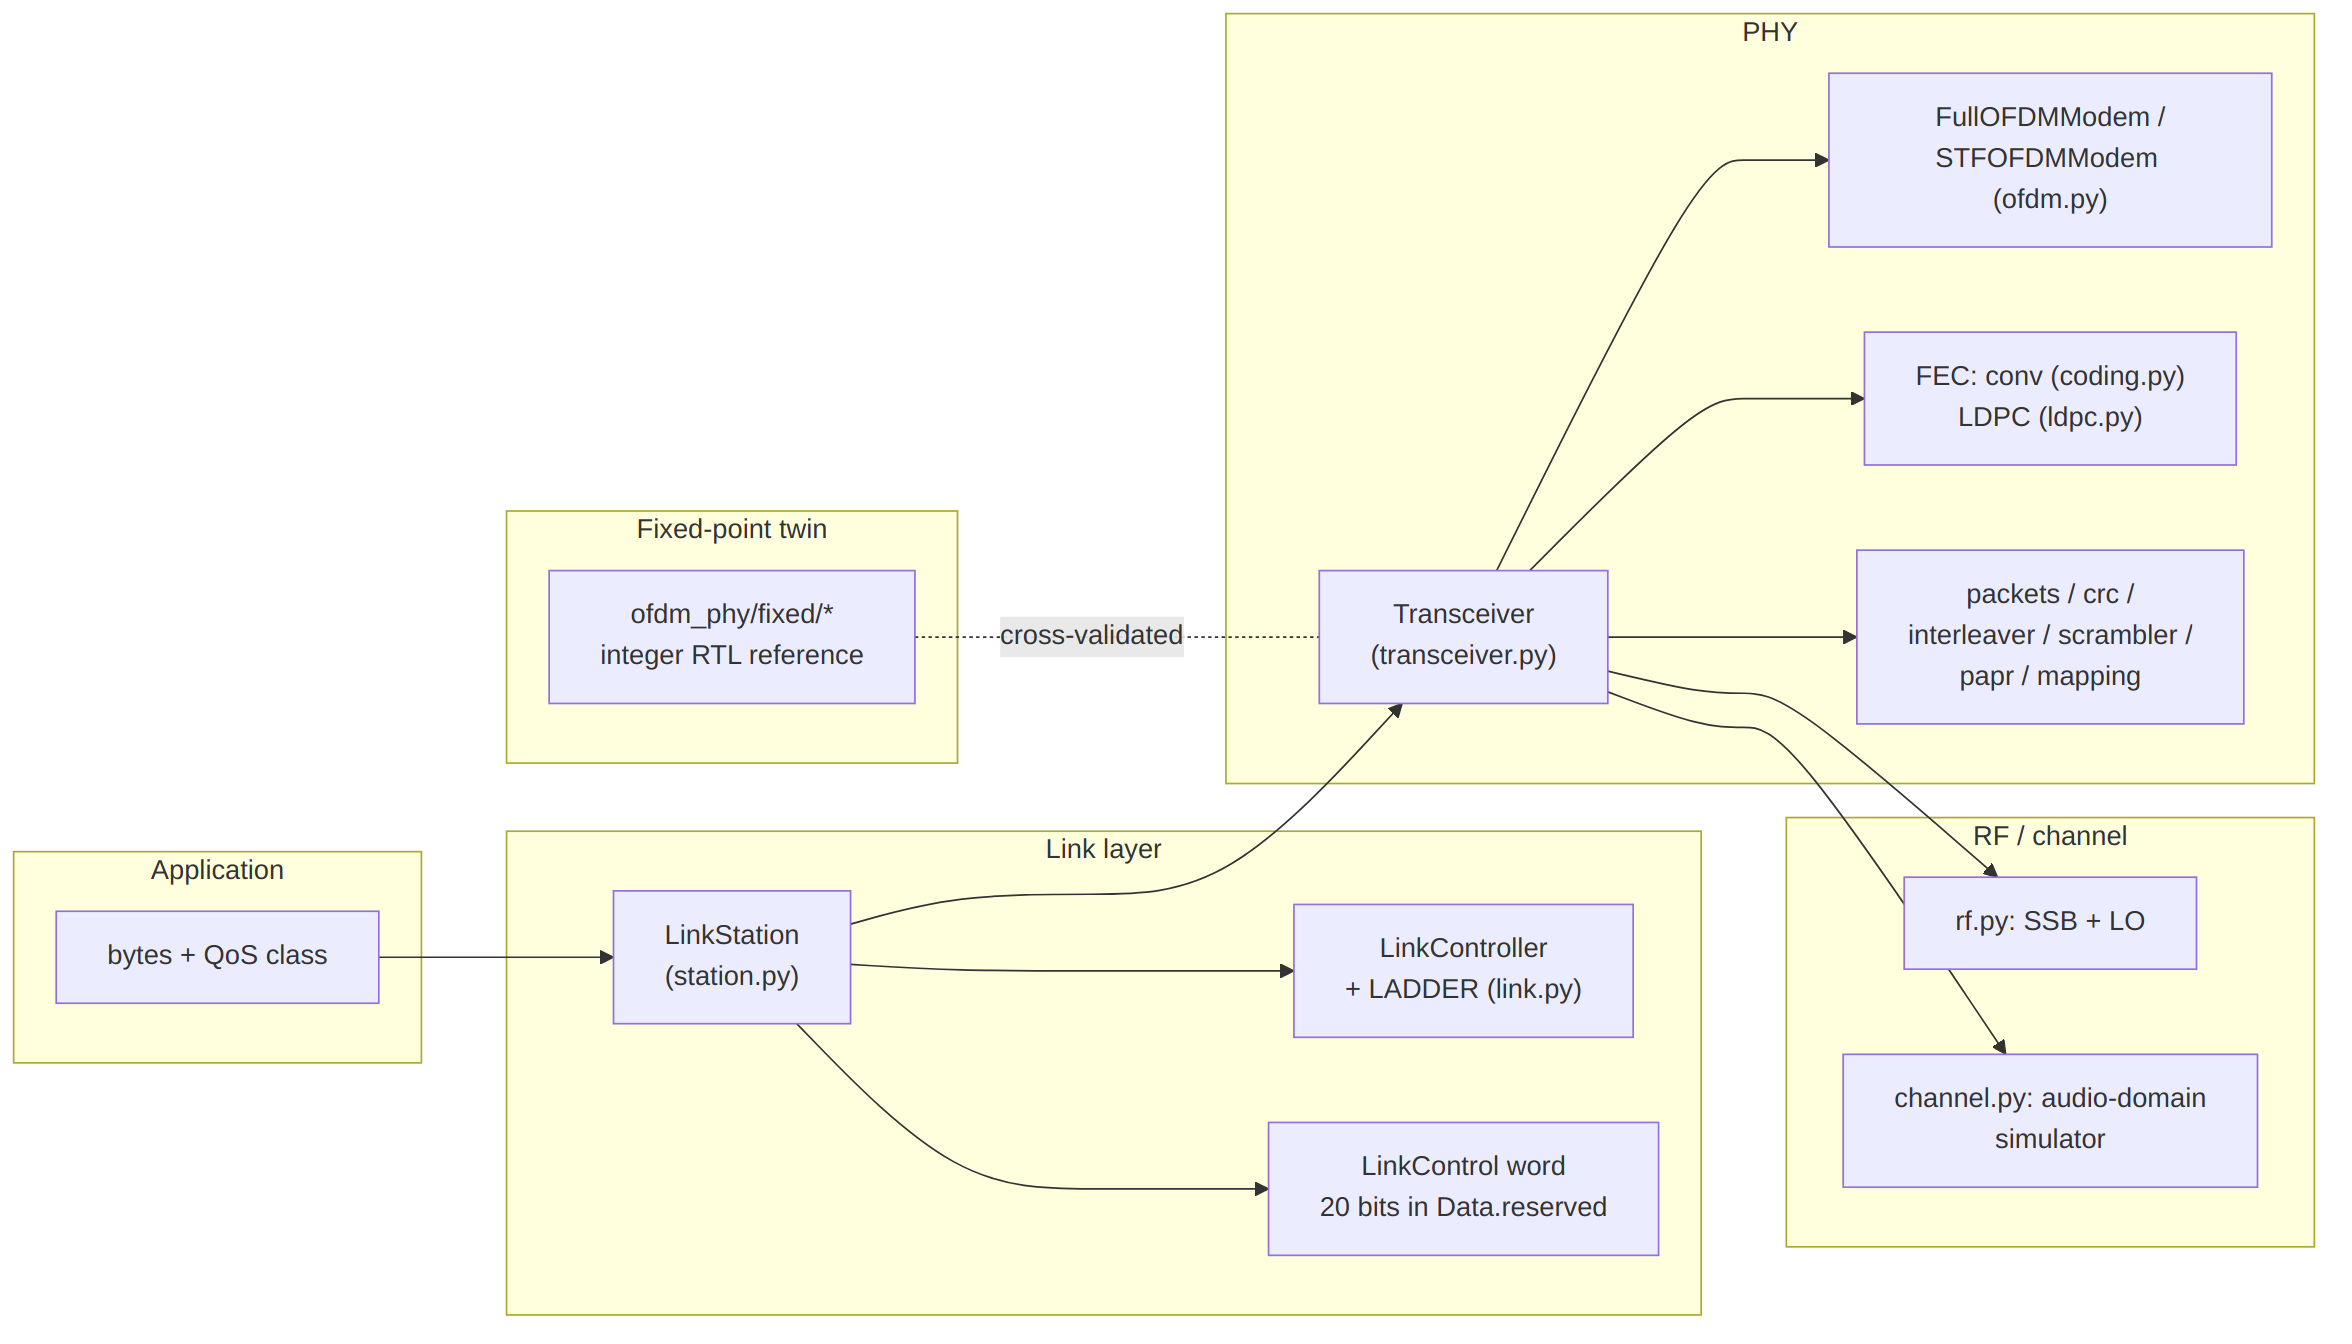
\includegraphics[width=\textwidth,height=0.55\textheight,keepaspectratio]{images/arch_layers.png}
    \caption{Layered architecture of the prototype.  The simulation-side
             layers (\texttt{channel.py}, \texttt{rf.py}) are exactly
             what a real deployment replaces with a soundcard and an SSB
             transceiver.}
    \label{fig:arch_layers}
\end{figure}

Three design principles shaped every layer.  First, \emph{faithful
defaults}: the plain \texttt{Transceiver} reproduces the article's
behaviour exactly (convolutional FEC, raw LLRs), and every improvement
--- LLR recalibration, LDPC coding, HARQ, AFC --- is opt-in and enabled
at the link layer, so the article-reproduction experiments remain valid
permanently.  Second, \emph{self-describing frames}: each link mode
owns a distinct Zadoff--Chu preamble root, so the receiver identifies
the mode from the preamble itself and a mode switch can never deadlock
the link.  Third, \emph{everything measured feeds back}: per-frame SNR
drives rate adaptation, per-frame CFO drives AFC netting, failed
decodes export their LLRs for HARQ combining, and every ACK or timeout
nudges learned per-rung sensitivity offsets.

\subsection{Scope of This Report}

This report documents the complete prototype in
\texttt{ofdm\_transceiver\_proto}: the article reproduction and its
verification, the synchronization analysis that closed the sensitivity
gap, every subsequent extension of the waveform and the link layer,
the two implementations that followed the Python model, and what the
system did on real hardware --- two boards on a wire, a
software-defined radio, and voice.  All quantitative claims are backed
by scripts in \texttt{experiments/} or by a bench target in
\texttt{cport/} (Section~\ref{sec:results}), and every one is
measured on a channel defined in Section~\ref{sec:channels}; the
measured artefacts (curves, JSON sweeps, WAV recordings) live in
\texttt{results/}.  Developer-oriented documentation with the same
structure exists as Markdown with Mermaid diagrams in \texttt{docs/}:
the layer documents (architecture, PHY, link, RF, fixed-point)
alongside four interface documents written for whoever implements
\emph{against} the system rather than inside it --- the channel
drivers, the two consoles, the USB transport, and the modem's
command/event model (Section~\ref{sec:cport_docs}).

\subsection{Contributions}

\begin{itemize}
    \item \textbf{Bit-exact article reproduction} --- 44/44 worked
          examples verified; BER/PER curves (article Figures~23--24)
          reproduced on the article's channel model; measured
          sensitivity $-7.2$\,dB versus the article's
          $\approx-7.5$\,dB, with the residual attributed to
          synchronization by a genie-synchronized control measurement.
    \item \textbf{Synchronization analysis and repair} --- three
          defects identified and fixed: the Zadoff--Chu
          time--frequency ambiguity ($\sim$1\,dB), an SNR-dependent
          tone-detection metric, and a preamble transmitted 7\,dB
          below data power.  An alternative 802.11-style preamble
          (proposed in the article's comment thread) was implemented
          and shown statistically equivalent.
    \item \textbf{SNR-adaptive modes} --- $16\times$ and $64\times$
          tiling modes with per-symbol residual-CFO hypothesis search,
          group-coherent ZC detection, and per-mode preamble roots,
          extending the sensitivity floor to $-17.9$\,dB (78\,\% of
          Shannon capacity at $-20$\,dB).
    \item \textbf{LLR recalibration} --- a measured monotone
          reliability map correcting a shape (not temperature)
          miscalibration of the demodulator's LLRs, worth 1.5--2\,dB
          at the BPSK/QPSK sensitivity edge.
    \item \textbf{Coding and modulation extensions} --- an IRA LDPC
          code (N=768, K=256) with normalized min-sum decoding,
          Gray-mapped 16-QAM extending the ladder to $+4.7$\,dB and
          1059\,bit/s, and CRC-gated chase-combining HARQ.
    \item \textbf{Adaptive link layer} --- a 13-rung measured rate
          ladder, receiver-driven adaptation over a 20-bit piggybacked
          link-control word, QoS with fragment-boundary preemption,
          stop-and-wait ARQ, and simplex channel access with carrier
          sense; validated by a whole-system two-station test with a
          mid-transfer fade.
    \item \textbf{AFC frequency netting} --- closed-loop carrier
          netting through the LC word ($+284$\,Hz initial offset
          converged inside a 12\,Hz deadband in five exchanges), with
          trim-budget and anchor guard rails against common-mode
          frequency drift.
    \item \textbf{RF-chain simulator} --- SSB modulator/product
          detector at a 48\,kHz IF rate with one shared reference
          oscillator per station, making CFO emerge physically from
          ppm errors and thermal drift (validated to 0.1\,Hz).
    \item \textbf{Fixed-point RTL reference model} --- an integer-only
          receiver covering the full frame family (conv+LDPC,
          BPSK/QPSK/16-QAM, all modes, HARQ, calibrated LLRs), within
          0.5\,dB of the float receiver at $-7$\,dB and ahead of it at
          $-9/-10$\,dB; its two-lag CFO unwrap recovered $\sim$8\,\%
          of all acquisitions that ARQ had been hiding.
    \item \textbf{Bit-exact C implementation on a microcontroller} ---
          the whole stack in C99 with no allocation and no floating
          point on the signal path, verified byte for byte against
          golden vectors; a streaming receiver whose memory follows the
          signal rather than the capture (10\,MB $\to$ 561\,KB, flash
          242 $\to$ 57\,KB); the EXTREME acquisition brought from
          not keeping up to 9.5\,\% of a 480\,MHz Cortex-M7 by
          measurement on the part; selective-repeat bursts, streamed
          windows, a capability handshake and operator ceilings ---
          68\,kB across the wire at 87\,\% of the raw rung-12 rate.
    \item \textbf{Two boards that are radios} --- flash-resident
          firmware with a 12\,kHz converter path, carrier sense with a
          DC-blind front end hardened by a stress campaign, a USB
          vendor-class modem protocol with a specification, and the
          field findings that shaped the link layer: a sentinel that
          crossed the air, a reply timer that had to learn the
          end-of-frame commit, a broadcast rung that decides who can
          hear it.
    \item \textbf{Adaptive broadcast} --- non-acknowledged delivery
          with a sender-signalled statistics exchange that re-rungs
          between blocks, proven on a fading harness ($+32$--39\,\% of
          the stream delivered against a held rung) and on the wire;
          a 73\,kB file byte-identical with 0 of 3089 frames lost.
    \item \textbf{Hosts on the link} --- a KISS TNC and an IP tunnel,
          each admitting traffic by air time rather than length; the
          SDR path with the transmitted spectrum, drive limits and an
          off-air decode measured; and a receive chain calibrated
          against a reference source.
    \item \textbf{Voice at 250\,bit/s} --- a neural codec evaluated
          for domain sensitivity, speaker identity, enrolment cost and
          streaming, then put on the air with push-to-talk between the
          boards: first audio 3.6\,s after the talker starts, decoded
          as it arrives, 24 of 24 transmissions lossless once a
          receiver commit defect the mode alone could expose was fixed.
\end{itemize}


\subsection{Signal Profile at a Glance}
\label{sec:signal_profile}

Table~\ref{tab:signal_profile} summarizes the on-air appearance of the
waveform in the style of a signal-identification database
entry~\cite{sigidwiki_vara}, for quick comparison with established
sound-card HF modes such as VARA~HF.

\begin{table}[H]
    \centering
    \caption{Signal identification profile (sigidwiki-style summary).}
    \label{tab:signal_profile}
    \small
    \begin{tabular}{@{}lp{9.2cm}@{}}
    \toprule
    \textbf{Field} & \textbf{Value} \\
    \midrule
    Frequency range   & any SSB voice channel (the waveform lives in the
                        300--2400\,Hz audio passband); amateur HF in the
                        source article's context \\
    Mode              & USB (audio passband, AGC off) \\
    Modulation        & OFDM, 23 subcarriers (16 data + 7 Zadoff--Chu
                        pilots), BPSK / QPSK / 16-QAM \\
    FEC               & convolutional $K{=}7$ rate 1/3 punctured to
                        1/2, 2/3, 3/4 (soft Viterbi); optional IRA LDPC \\
    Bandwidth         & $\approx$2.1\,kHz occupied (bins 3--25 at
                        93.75\,Hz spacing) \\
    Symbol rate       & 22.1 / 5.8 / 1.46\,symbols/s
                        (NORMAL / ROBUST / EXTREME tiling) \\
    ACF               & 10.7\,ms (intra-symbol tile);
                        45.3 / 173 / 685\,ms (symbol, mode-dependent) \\
    Net data rate     & 7.8--1059\,bit/s, 13-rung adaptive ladder
                        (Table~\ref{tab:ladder}) \\
    Sensitivity       & down to $-17.9$\,dB SNR (noise in the 6\,kHz
                        Nyquist band; $\approx-14$\,dB re 2.5\,kHz) \\
    Identification    & three-part preamble: two Newman-phased tone
                        combs, then a tiled Zadoff--Chu symbol whose
                        root (17/19/21) labels the link mode; the
                        EXTREME bootstrap is heard as a
                        $\approx$21\,s steady warble \\
    Duplex / access   & simplex; carrier sense, stop-and-wait ARQ with
                        selective-repeat streamed bursts, capability
                        handshake, and a non-acknowledged broadcast
                        mode (Sections~\ref{sec:link},
                        \ref{sec:broadcast}) \\
    Status            & research prototype (this work): simulation,
                        two-board wire stand, and an off-air decode
                        through an SDR at 7\,MHz; not a deployed
                        on-air standard \\
    Short description & audio-band adaptive OFDM data modem for SSB
                        transceivers, reproducing and extending the
                        PHY of~\cite{habr_ofdm} \\
    \bottomrule
    \end{tabular}
\end{table}

\subsection{Report Structure}

Section~\ref{sec:channels} defines the conventions and the six
channels --- three simulated, one wired, one radio, one a family of
harnesses --- on which everything that follows was measured, and maps
each headline result to its channel.

Part~\ref{part:phy} is the physical layer.
Section~\ref{sec:phy} describes the PHY as implemented;
Section~\ref{sec:sync} the synchronization analysis that closed the
sensitivity gap; Section~\ref{sec:modes} the SNR-adaptive link modes;
Section~\ref{sec:llr} LLR quality measurement and recalibration; and
Section~\ref{sec:coding} the LDPC, 16-QAM and HARQ extensions.

Part~\ref{part:link} is the link layer.  Section~\ref{sec:link}
covers the rate ladder, the link-control word, adaptation, ARQ and
QoS, burst windows, the reply timer, simplex access, the capability
handshake and AFC netting; Section~\ref{sec:broadcast} the broadcast
mode, from its design on the simulated channels to the statistics
exchange the boards required.

Part~\ref{part:impl} is the implementations and what they did.
Section~\ref{sec:fixed} is the fixed-point RTL reference model;
Section~\ref{sec:cport} the C implementation as engineering ---
bit-exactness, the streaming receiver, memory and processor budgets,
hardening; Section~\ref{sec:radio} the radio firmware and the
two-board stand; Section~\ref{sec:host} the USB interface and the host
tools; Section~\ref{sec:cport_sdr} the SDR path; and
Section~\ref{sec:cport_voice} voice at 250\,bit/s, evaluated and then
on the air.

Part~\ref{part:results} consolidates.  Section~\ref{sec:results}
collects the regression suites, the measured gains and the
demonstrations; Section~\ref{sec:discussion} discusses what binds
performance, the limitations and the work ahead; and
Section~\ref{sec:conclusion} concludes.
